\chapter{Implémentation}
\section{Transformation CAN/CNA}
%can
Afin de réalisé notre commande, nous avons dût transformer la valeur entière lue pour $V_S$ par le CAN en un équivalent de la tension de type nombre à virgule flottante.  Figure \ref{fig:CAN_p}, nous pouvons observer les valeurs que peut convertir le CAN et les valeurs dont nous avons besoins. Nous n'utilisons ici que la moitié de la valeur lue par le convertisseur car nous n'avons besoin de convertir que des valeurs comprises entre $0$ et $5$ Volt. Ici, la plage de conversion est donc à moitié utilisée. 
Dans un premier temps, nous avons décaler la valeur lue (avec un et bit a bit) afin d'avoir la valeur sur $\left[ 0 , 1023\right]$ (équation \ref{equ:CAN1}) puis  nous avons réalisé la conversion en tension avec l'équation \ref{equ:CAN}.
\begin{eqnarray}
\label{equ:CAN1}V_{CANr} &=& V_{CAN} \&_{bàb} 1023\\
\label{equ:CAN}V_{volt} &=& \frac{5}{2^{10}-1}V_{CANr}
\end{eqnarray}
%%cna
La génération de la sortie $V_M$ nécessite aussi une conversion du CNA depuis la tension calculée par la commande (nombre à virgule flottante) vers un entier compris entre $-5$ et $5$ Volts. Néanmoins, la commande calcule une valeur comprise entre $-5$ et $5$ Volts, mais la carte de puissance branchée sur la sortie du CNA nécessite en entrée une tension comprise entre $0$ et $5$ Volt. Il faut donc, dans un premier temps, redresser la valeur calculée $V_{com}$ par la sortie sur une intervalle $\left[0;5\right]$ $V_{redr}$, puis le convertir en entier $V_{CNA}$. Pour cela nous utilisons les équations suivantes :
\begin{equation}
\begin{array}{lcl}
V_{red}	&=&	\frac{1}{2}V_{com}+2,5\\
V_{CNA} &=& \frac{10}{2^{12}-1}V_{red}-5\\
V_{CNA} &=& \frac{V_{com}}{819} - \frac{4090}{819}
\end{array}
\end{equation}	
\begin{figure}[!ht]%
\begin{minipage}{.5\textwidth}%
\centering
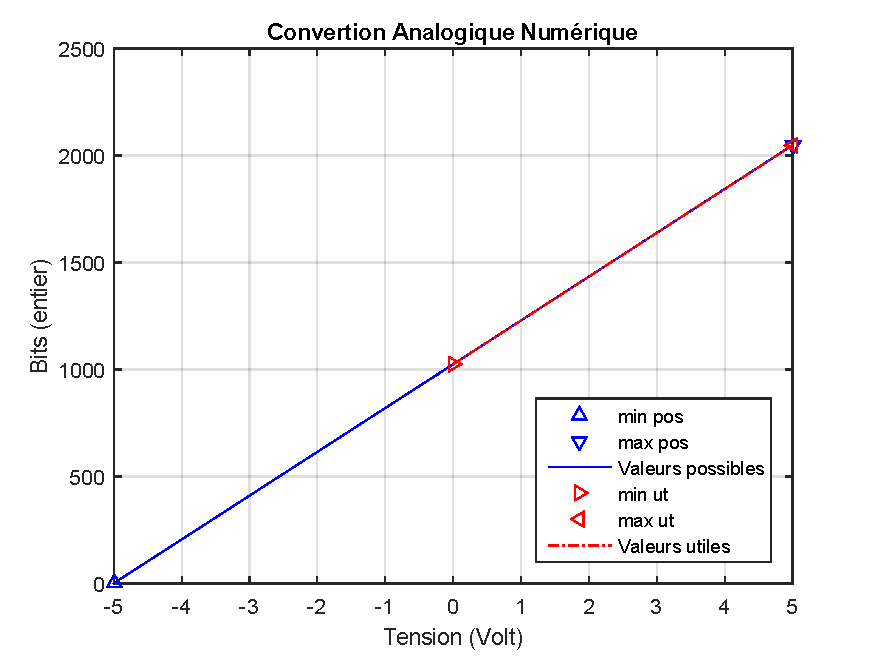
\includegraphics[width=\textwidth]{./VI/images/CAN_plage.pdf}
\caption{\label{fig:CAN_p}Valeurs possibles et possibles du CAN}
\end{minipage}%
\hfill%
\begin{minipage}{.5\textwidth}%
\centering
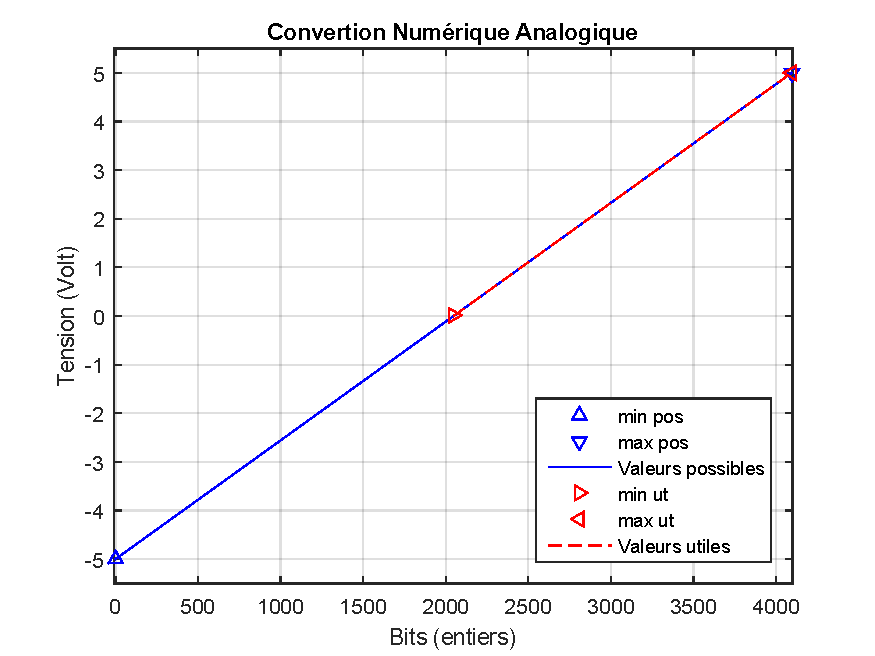
\includegraphics[width=\textwidth]{./VI/images/CNA_plage.pdf}
\caption{\label{fig:CNA_p}Valeurs possibles et possibles du CNA}
\end{minipage}%
\end{figure}

%	\subsection{Implémentation d'un programme de test des convertisseurs}
%	\subsection{Correction}
\section{Implémentation}
		\subsection{Description des taches}
		\subsection{implémentation}
		\subsection{Validation et correction}